\subsection{Model Identification}
\label{subsec:Identification}

\begin{frame}{Implementation - World model}

    \begin{figure}[h]
    \centering
    
\includegraphics[width=10cm]{Figures/code_structure_world_model.png}
    \caption{The nodes, inputs and outputs that make up the code.}
    \label{fig:code_struct}
    \end{figure}
    		
\end{frame}

\begin{frame}{Model Identification}
\tikzstyle{int}=[draw, fill=black!0, minimum size=2em]
\tikzstyle{tf}=[draw, fill=black!0, minimum size=2em]
\tikzstyle{init} = [pin edge={to-,thin,black}]
\tikzstyle{input} = [coordinate]
\tikzstyle{output} = [coordinate]

\begin{figure}
    \centering
    \resizebox{0.7\linewidth}{!}{%
\begin{tikzpicture}[node distance=3cm,auto,>=latex']
    \node [tf, name=input] (a) {Drone};
    \node (b) [left of=a,node distance=3cm, coordinate] {a};
    \node [int] (c) [right of=a] {$\int$};
    \node [coordinate] (end) [right of=c, node distance=3cm]{};

    \path[->] (b) edge node {$j_x$,$j_y$,$j_z$} (a);
    \draw[->] (a) edge node {$v_x$,$v_y$,$v_z$} (c);
    \draw[->] (c) edge node {$p_x$,$p_y$,$p_z$} (end);
\end{tikzpicture}
}
    % \caption{Block diagram}
    \label{fig:ideal_cont_model}
\end{figure}
    
    \vspace{4mm}
    
    \begin{equation*}
    H_{XJ}(s) = \frac{X_{x,y}(s)}{J_{x,y}(s)} = \frac{b_0}{s^3 + a_2 s^2 + a_1 s + a_0}
    \label{eq:pos_tf_3dorder}
    \end{equation*}

    \begin{equation*}
    H_{VJ}(s) = \frac{V_{x,y}(s)}{J_{x,y}(s)} = \frac{b_0}{s^2 + a_1 s + a_0}
    \label{eq:vel_tf_2ndorder}
    \end{equation*}
    
    \vspace{4mm}
    $\rightarrow$ Least-squares discrete time domain parameter identification
    
\end{frame}

\begin{frame}{Identification experiment - X, Y}

\begin{figure}[h]
    \vspace{-3.4mm}
    \centering
    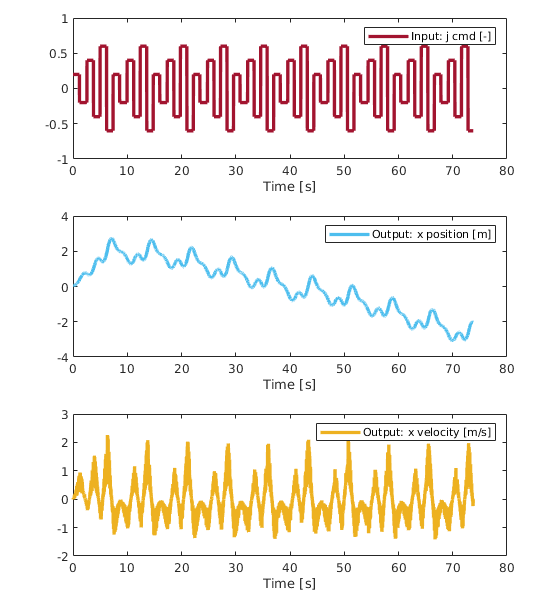
\includegraphics[height=7.7cm]{Figures/X_pos_vel_input_output.png}
    % \caption{}
    \label{fig:coord_frame}
    \end{figure}
    
\end{frame}

\begin{frame}{Identification results - X, Y}

\begin{figure}[h]
    % \vspace{-3.4mm}
    \centering
    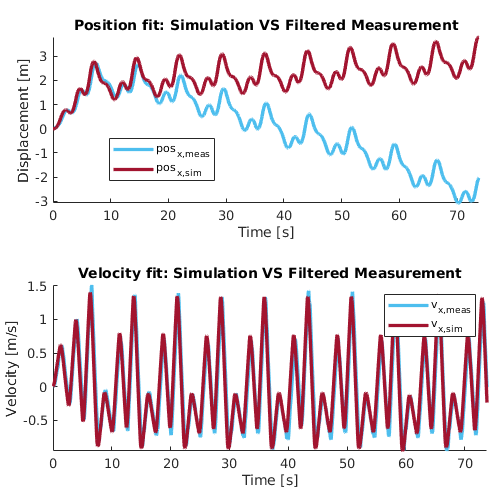
\includegraphics[height=7.7cm]{Figures/X_pos_vel_fit_result.png}
    % \caption{}
    \label{fig:coord_frame}
    \end{figure}
    
\end{frame}